\documentclass[paper=a4, fontsize=11pt, UTF8]{article} % A4 paper and 11pt font size
\usepackage[a4paper,left=3.18cm,right=3.18cm,top=2.5cm,bottom=2.5cm]{geometry}
\usepackage{ctex}
%\usepackage[T1]{fontenc} % Use 8-bit encoding that has 256 glyphs
%\usepackage{fourier} % Use the Adobe Utopia font for the document - comment this line to return to the LaTeX default
\usepackage[english]{babel} % English language/hyphenation
\usepackage{amsmath,amsfonts,amsthm} % Math packages
\usepackage{graphicx}
%\usepackage{rotating} % for sidewaysfigure
\usepackage{listings}
\usepackage{xcolor}
\usepackage{siunitx}
\usepackage{booktabs}
\usepackage{multirow}
\usepackage{longtable}
\usepackage{hyperref}
\hypersetup{
    colorlinks,
    citecolor=black,
    filecolor=black,
    linkcolor=black,
    urlcolor=black
}

% Uncomment below to New page befor section
%\usepackage{titlesec}
%\newcommand{\sectionbreak}{\clearpage}
%\titleformat*{\section}{\centering \Large \bfseries}

\newcommand{\matr}[1]{\mathbf{#1}} % undergraduate algebra version
%\usepackage{sectsty} % Allows customizing section commands
%\allsectionsfont{\centering \normalfont\scshape} % Make all sections centered, the default font and small caps

\usepackage{fancyhdr} % Custom headers and footers
\pagestyle{fancyplain} % Makes all pages in the document conform to the custom headers and footers
\fancyhead[L]{}
\fancyhead[C]{}
\fancyhead[R]{\thepage} % No page header - if you want one, create it in the same way as the footers below
\fancyfoot[L]{} % Empty left footer
\fancyfoot[C]{\thepage} % Empty center footer
\fancyfoot[R]{} % Page numbering for right footer
%\renewcommand{\headrulewidth}{0pt} % Remove header underlines
\renewcommand{\footrulewidth}{0pt} % Remove footer underlines
\setlength{\headheight}{13.6pt} % Customize the height of the header

\numberwithin{equation}{section} % Number equations within sections (i.e. 1.1, 1.2, 2.1, 2.2 instead of 1, 2, 3, 4)
\numberwithin{figure}{section} % Number figures within sections (i.e. 1.1, 1.2, 2.1, 2.2 instead of 1, 2, 3, 4)
\numberwithin{table}{section} % Number tables within sections (i.e. 1.1, 1.2, 2.1, 2.2 instead of 1, 2, 3, 4)

%\setlength\parindent{0pt} % Removes all indentation from paragraphs - comment this line for an assignment with lots of text

\lstset{language=C++,%
    %basicstyle=\color{red},
    keywordstyle=\color{blue},%
    extendedchars=false,
    tabsize=4,
    breaklines,
    morekeywords=[2]{1}, keywordstyle=[2]{\color{black}},
    identifierstyle=\color{black},%
    stringstyle=\color{mylilas},
    commentstyle=\color{green},%
    frame=single,
    showstringspaces=false,%without this there will be a symbol in the places where there is a space
    numbers=left,%
    numberstyle={\small \color{black}},% size of the numbers
    numbersep=9pt, % this defines how far the numbers are from the text
    emph=[1]{for,end,break},emphstyle=[1]\color{red}, %some words to emphasise
    escapeinside=``
}


%\usepackage[framed,numbered,autolinebreaks,useliterate]{mcode}

\newcommand{\horrule}[1]{\rule{\linewidth}{#1}} % Create horizontal rule command with 1 argument of height

\title{
\normalfont \normalsize
\textsc{\kaishu 网络专题训练} \\ [5pt] % Your university, school and/or department name(s)
\horrule{0.5pt} \\[0.4cm] % Thin top horizontal rule
\huge 4over6隧道协议实验报告 \\ % The assignment title
\horrule{2pt} \\[0.5cm] % Thick bottom horizontal rule
}

\author{马 \;  也\quad 2013011365 \quad 计34\\ 沈哲言\quad 2013011371 \quad 计34}
%\author{马也} % Your name
\date{\normalsize\today} % Today's date or a custom date

\begin{document}

\maketitle % Print the title

% \thispagestyle{empty}
% \newpage

%\setcounter{page}{1}
%\tableofcontents
\fontsize{11pt}{18pt}\selectfont
%\newpage

\section{实验目的}

\begin{itemize}
\item 掌握Android下应用程序开发环境的搭建和使用
\item 掌握IPv4 over IPv6隧道的工作原理
\end{itemize}


\section{实验原理}

\subsection{4over6隧道模式原理}

\begin{figure}[htp]
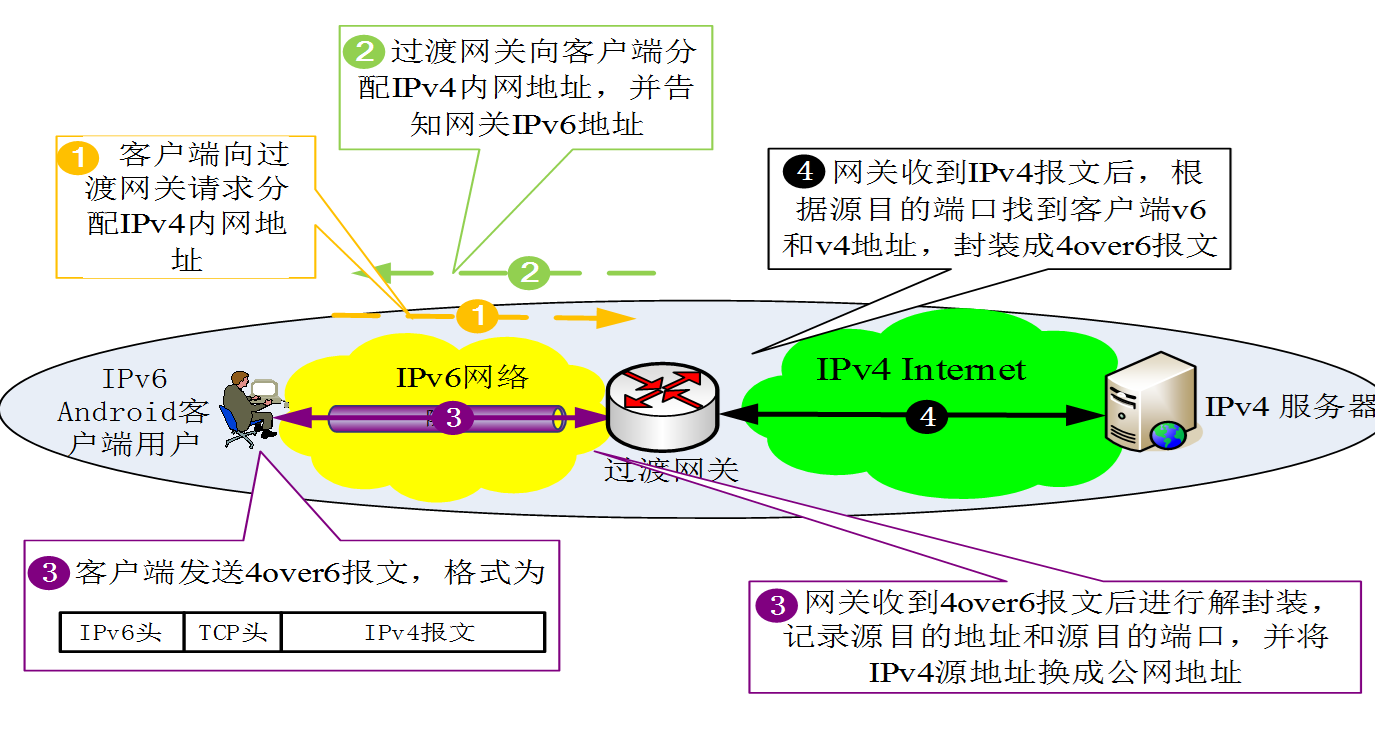
\includegraphics[width=\textwidth]{fig1}
\caption{4over6隧道模式原理图}
\end{figure}

IPv4 over IPv6隧道模式是指,将IPv4的报文装载到IPv6网络的数据段,通过隧道模式进行传递,这样就可以使用IPv6的网络来访问IPv4的资源。主要流程如下:

安卓客户端向过渡网关请求分配IPv4内网地址;过渡网关分配IPv4内网地址,并提供对应的IPv6网络地址;接着,安卓客户端发送4over6报文,过渡网关接受报文并进行分析,得到源地址和目的地址,将IPv4地址转化为公网地址,发送到公网之中;当过渡网关收到公网的IPv4报文之后,根据记录好的映射关系,重新封装成4over6报文,发给对应的内网用户,完成数据的转发和接受。

在以上流程中,用户处于IPv6的网络环境之中,过渡网关横跨IPv4和IPv6,并在其中提供IPv4和IPv6地址的转换和分发。在本实验中,过渡网关部分的代码已经完成,我们需要完成用户端的代码,以实现IPv4 over IPv6隧道协议。

\subsection{安卓VPN Service原理}

在本实验中,我们采用了VPN Service作为基本框架来实现IPv4 over IPv6隧道协议。VPN Service是安卓提供的一套API接口,方便编程人员创建VPN服务。当打开该服务之后,安卓系统将所有应用程序发送的IP包都根据iptables,使用NAT转发到TUN虚拟网络设备上,其端口为tun0。当打开VPN Service之后,我们可以获取tun0的文件描述符,这样就可以读取或者写入数据以实现发送或者接收数据。

也就是说,在打开VPN Service之后,我们可以监控系统所有的网络进程,并从tun中获得系统中所有IP包。这样,我们就可以将IP包封装在IPv6报文之中,使用隧道协议将报文发送到服务器,实现数据的发送;当我们收到服务器反馈的IPv6报文后,我们将其进行拆解,得到真正的IPv4包,再写入到tun文件之中,以实现数据的接收。

\subsection{JNI与NDK}

在本次实验中,由于经常要和以字节为单位的数据打交道,并且需要精细地管理内存,因此我们采用C来实现IPv4 over IPv6的核心功能。要在以Java为语言的安卓环境中使用C来进行编程,我们需要使用JNI和NDK。

Java Native Interface(JNI)规定了一套Java的原生接口,规定了Java和其他语言交互或者是在其他平台下运行时的接口,让我们可以使用其他语言(如C、C++、汇编等)访问Java中的类和对象。而Native Development Kit(NDK)是Google提供的一套方便开发者的开发套装(SDK),方便编程人员将C或者C++程序打包并加入到APK之中,供安卓程序使用。

\section{实验设计与内容}

\subsection{程序整体设计流程}

本次实验的编码主要分为两个部分,Java实现的安卓客户端(前端)和C实现的收发进程(后端),前端和后端之间通过管道(named pipe)来进行连接并传递数据。实验整体流程如下:

\begin{figure}[htp]
\center
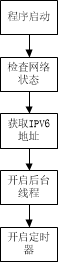
\includegraphics[scale=1]{fig2}
\caption{整体工作流程}\label{fig2}
\end{figure}


\subsection{前端工作流程}

\subsubsection{工作流程}

\begin{figure}[htp]
\center
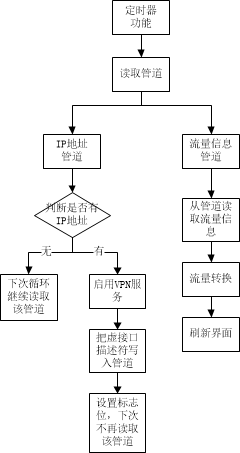
\includegraphics[scale=0.9]{fig4}
\caption{前端工作流程}\label{fig4}
\end{figure}

\newpage 

前台流程如上图所示,前台的前台定时器主要功能为定时刷新显示界面,显示流量信息,定时器功能解析如下:

\begin{enumerate}
\item 开启定时器之前,创建一个读取IP信息管道的全局标志位flag,默认置0;
\item 开始读取管道,首先读取IP信息管道,判断是否有后台传送来的IP等信息;
\item 假如没有,下次循环继续读取;
\item 有IP信息,就启用安卓VPN服务(此部分在后面有详细解释);
\item 把获取到的安卓虚接口描述符写入管道传到后台;
\item 把flag置1,下次循环不再读取该IP信息管道;
\item 读取流量信息管道;
\item 从管道读取后台传来的实时流量信息;
\item 把流量信息进行格式转换;
\item 显示到界面;
\item 界面显示的信息有运行时长、上传和下载速度、上传总流量和包数、下载总流量和包数、下联虚接口V4地址、上联物理接口IPV6地址。
\end{enumerate}

\subsubsection{具体实现}

这一部分主要包括了安卓APP界面的实现、UI主线程、VPN服务、后台定时器刷新线程以及后台C线程的实现。

\paragraph{界面:} 界面使用了安卓开发中较为常用的LinearLayout来实现主界面,在界面上布局了两个Button(分别用于启用和终止服务)以及六个TextView(分别显示服务持续时间、上传下载速度、上传下载流量和IP信息等等)

\paragraph{UI主线程:} MainActivity的主要任务是初始化全局的变量、启动两个后台的线程并打开VPN服务。首先主线程通过getLocalIpAddress函数获取本机的IPV6地址,只有成功获取到地址才会继续后续的服务。其次为启动服务按钮注册监听事件,若按下则会启动两个后台的线程IVI和BackGround。

\paragraph{IVI线程:} 通过JNI调用后台的C函数启动后台C线程;

\paragraph{BackgGround线程:} 这个线程的工作比较多,首先它需要连接IP信息的管道(由后台C线程负责创建),接收来自C线程的虚接口的IPV4地址,然后启动VPN服务,并把TUN的文件描述符通过管道传回C线程;最后启动定时器服务例程刷新页面。

\paragraph{VPN服务:} 继承一个VpnService的类,根据传入的参数(IP地址,DNS服务器等等)初始化Vpn服务并启动,获取到TUN虚接口的文件描述符后,通过管道传回C线程

\paragraph{ 定时器刷新例程:}集成了java.util.TimerTask类,连接了后台C线程创建的流量信息管道,进行一定的格式转换之后显示在界面上。

\newpage
\subsection{后端工作流程}

\subsubsection{工作流程}

\begin{figure}[htp]
\center
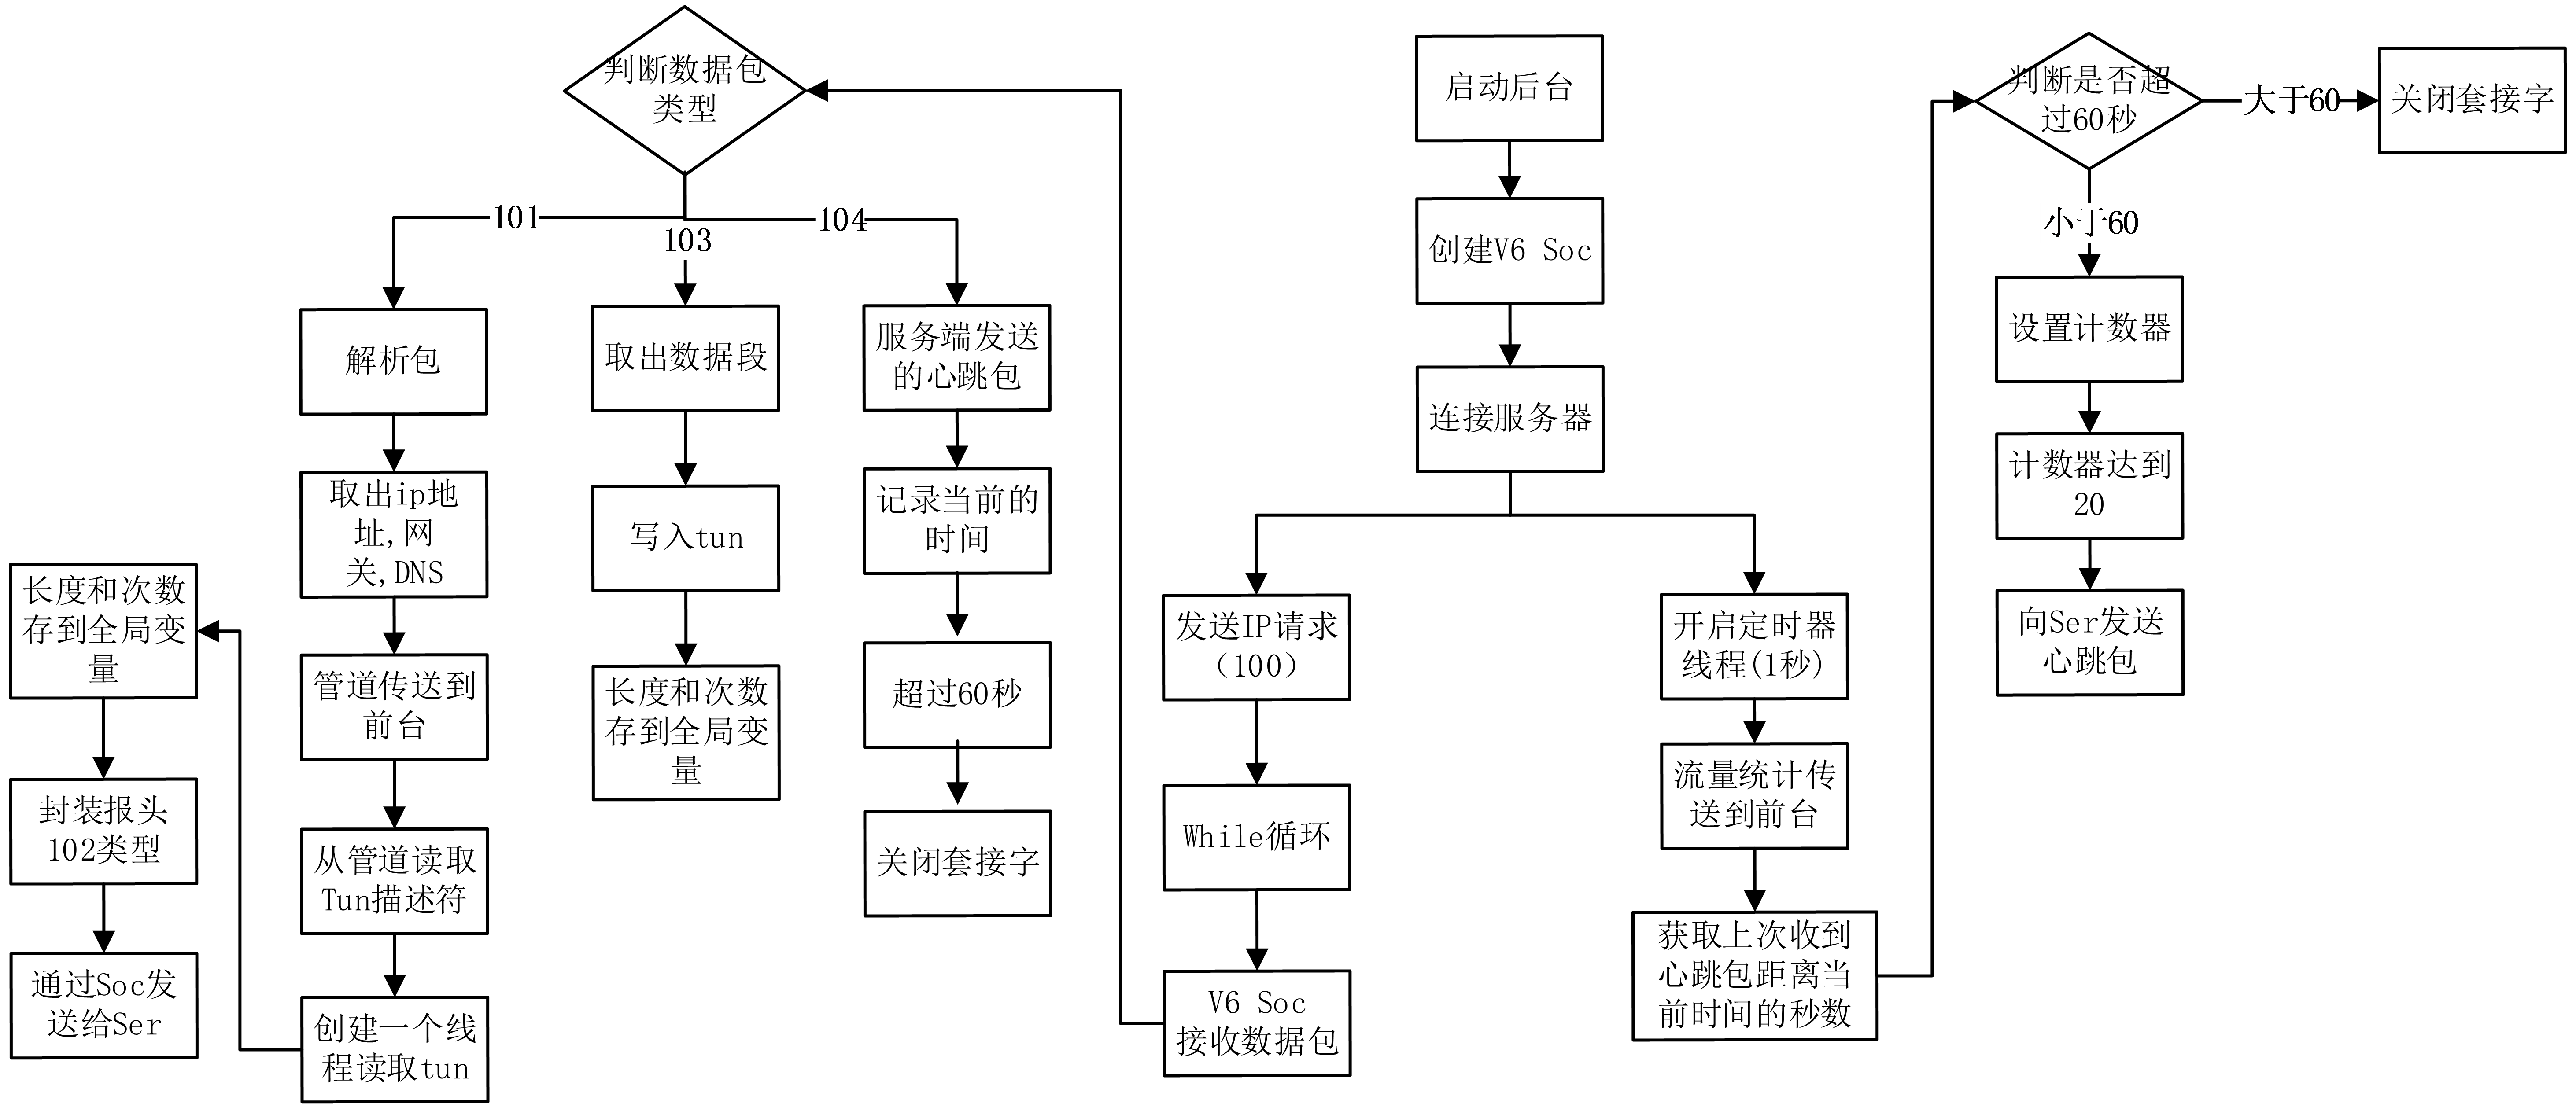
\includegraphics[width=\textwidth]{fig3}
\caption{后端工作流程}\label{fig3}
\end{figure}

\begin{enumerate}
\item 创建IPV6套接字;
\item 连接4over6隧道服务器;
\item 开启定时器线程(间隔1秒):
\begin{enumerate}
\item 读写虚接口的流量信息写入管道;
\item 获取上次收到心跳包距离当前时间的秒数S;
\item 假如S大于60,说明连接超时,就关闭套接字;
\item S小于60就每隔20秒给服务器发送一次心跳包。
\end{enumerate}
\item 发送消息类型为100的IP请求消息;
\item while循环中接收服务器发送来的消息,并对消息类型进行判断;
\begin{enumerate}
\item 101类型(IP响应):
\begin{enumerate}
\item 取出数据段,解析出IP地址,路由,DNS;
\item 把解析到的IP地址,路由,DNS写入管道;
\item 从管道读取前台传送来的虚接口文件描述符;
\item 创建读取虚接口线程:
\begin{enumerate}
\item 持续读取虚接口;
\item 记录读取的长度和次数;
\item 封装102(上网请求)类型的报头;
\item 通过IPV6套接字发送给4over6隧道服务器。
\end{enumerate}
\end{enumerate}
\item 103类型(上网应答):
\begin{enumerate}
\item 取出数据部分;
\item 写入虚接口;
\item 存下写入长度和写入次数。
\end{enumerate}
\item 104类型(心跳包):
\begin{enumerate}
\item 记录当前时间到一个全局变量。
\end{enumerate}
\end{enumerate}
\end{enumerate}

\subsubsection{具体实现}


后端使用C语言SOCKET编程实现的,其有一个主函数main用于Java线程执行,其主要流程参见图 \ref{fig3},主要阐述如下:

首先,创建和服务器连接时使用的Socket,并进行地址绑定,建立TCP连接。注意这里创建的是IPv6的Socket,创建和连接方法为:

\begin{verbatim}
client_socket = socket(AF_INET6, SOCK_STREAM, 0);

server_socket.sin6_family = AF_INET6;
server_socket.sin6_port = htons(SERVER_PORT);
inet_pton(AF_INET6, SERVER_ADDR, &server_socket.sin6_addr);

connect(client_socket, (struct sockaddr *) &server_socket,
        sizeof(server_socket));
\end{verbatim}

以上代码创建了客户端Socket,绑定了服务器地址,并进行TCP连接,其中\texttt{AF\_INET6}指明是IPv6,\texttt{SOCK\_STREAM}指明是TCP连接。

连接成功之后,新建一个定时器线程\texttt{timer\_thread},用于每次隔1s执行一次操作,其主要负责:每秒给前端发送统计数据,每20s给服务器发送心跳包,每秒检查服务器心跳包是否超时(60s)。发送的统计数据包括这1s内接受数据包的数量、发送数据包的数量、接受数据包的总大小、发送数据包的总大小。

回到主函数,在连接成功之后,向服务器发送第一个IP请求包\texttt{IP\_REQ},然后开始循环等待服务器回应:

\begin{verbatim}
while(!isClosed) {
	// Receive Package

	// Parse Package

	if(!hasIP && msg.type == MSGTYPE_IP_REC) {
		// Receive IP
	}
	else if(msg.type == MSGTYPE_DATA_RECV) {
		// Receive data and update stats
	}
	else if(msg.type == MSGTYPE_HEARTBEAT) {
		// Update heart beat time to now
		heartbeat_recv_time = time((time_t*)NULL);
	}
	else {
		// Unknown
	}
}
\end{verbatim}

收到的包分为三个类别:收到IP包,收到数据包,收到心跳包。下面分别进行阐述:
\paragraph{IP\_REC} \mbox{}\\
当收到IP包,就证明和服务器的连接已经建立好了,这时候需要依次完成如下步骤:写入\texttt{IP\_REC}中的数据到管道之中,从管道中读取tun文件句柄号,创建新的线程循环读取tun文件。由于C语言中字符串处理操作较为复杂,故对\texttt{IP\_REC}包中的数据不做处理直接发送给Java,由前端获取每一段的信息,开启VPN Service。对于tun文件,前端只需要给后端发送其句柄号(在Linux系统中每个进程中每个打开的文件都有其特有且唯一的句柄号),后端就可以对这个tun文件进行读写了。因此,最后创建新的线程循环读取tun文件的内容。

在读取tun文件的时候,有一个小的优化,为了不让循环检查read始终阻塞进程“忙等”,这里使用Linux中的select函数进行“闲等”,具体可以参阅Linux中select函数的文档。

\paragraph{DATA\_REC} \mbox{}\\
当收到数据包,就代表收到了服务器转发的数据,这时候直接将其data字段写入tun文件之中即可,并更新统计信息。更新统计信息时需要注意加锁操作,防止竞争问题。

\paragraph{HEARTBEAT} \mbox{}\\
当收到心跳包的时候,更新收到心跳包的时间即可(因为心跳包的发送和超时检查在定时器线程)。


\section{实验结果与分析}

在本实验的测试过程中,使用了安装了安卓系统的华为手机进行了测试,网络环境为在寝室用极路由搭建的Ipv6局域网环境。在手机开启了VPN服务之后,我们测试了各种传输对象和传输环境,包括但不限于:内网环境下的Info站点的图片及文字;外网环境下百度首页、阅读、图片等各种百度服务(浏览器端),微信文字聊天、图片、小视频发送以及视频通话功能(客户端);以及一些APP的后台推送功能。

通过测试,我们发现手机的上网功能基本可用,说明了我们的VPN服务功能和4 over 6实现基本正确。在IPv6网络稳定的情况下,打开info主页这种文字较多的网页所用的延迟大概为一到两秒,这说明了我们实现的高效性;在测试微信视频聊天的时候,我们发现手机收到的视频图像几乎没有卡顿,仅仅是发送出去的视频有略微的卡顿,这也证明了我们实现的高效与鲁棒。

\newpage
\section{实验中遇到的问题}

在实验中,我们主要遇到了三个比较大的问题。

第一个问题是,当我们后端C代码和前端VPN Service结合在一起之后,就发送不出去心跳包了。经过调试,我们发现是开启VPN Service之后,原来创建的C的socket也会被导入到tun文件中,这就形成了自环。解决方法比较简单,我们使用安卓中提供的protect函数保护之前建立好的socket就可以了。至于这个socket则通过一开始的named pipe和着IP地址一并传送到前端即可。

第二个问题是,在编码完毕后,我们在调试信息中发现,经常有类型不等于预设的几种类型的报文,并且这些报文之前一定紧跟着一个最大长度的报文,也就是说,IPv4报文在传输的过程中被截断了。由于我们和服务器之间的通信没有size和offset等设置,所以一旦被截断也不可能在客户端进行拼接和恢复。这就导致了我们在一开始测试微信发送图片以及视频聊天时速度奇慢,几乎不能正常使用,打开info网页至少需要5-6秒才能打开,并且图片几乎加载不出来。

为了解决这个问题,我们尝试了许多办法,包括设置MTU长度为小于1500的一个值,发现几乎没有改变。另外,我们还尝试接收时不一次性接收完,而是持续接收,直到接收size个字节才停止,但是也没有明显地改善。最后,我们发现,首先接受4个字节(size),然后接受size次,每次一个字节,这样的操作可以极大减少报文被分拆的可能,提高有效传输速度,所以我们最后采用了这种做法,也得到了实验的证实。

第三个问题是有关于UI线程阻塞的问题,UI线程作为维护安卓界面的主线程,在其中不应该设置非常多耗时且有可能阻塞的操作,在和管道交互时如果将读取等操作放在主线程很有可能导致界面的阻塞,故应该新增一个线程进行IO操作并刷新界面。


\section{实验心得与体会}

在这次实验中,我们掌握了Android下应用程序开发环境的搭建和使用,理解了4over6的原理,并实现了一个测试通过,效果良好,具有鲁棒性的4over6安卓APP。除此之外,我们对于原理课上所讲的4over6又有了更深的理解和体会,并通过自己的切身实践,锻炼和编码能力,深化了对于转发、隧道等概念的理解,达到了该大实验的目的。

\section{对实验的意见和建议}

本实验有效锻炼了同学们的编码能力和实践能力,但是我们认为还存在些许的瑕疵。根据我们的完成情况,前端同学几乎只需要做一个Activity界面,并学习Android VPN Service部分文档即可,后端同学则只是涉及到socket编程和一些简单的C语言知识,后端全部代码加起来不过300行左右。代码编写时间也不会太长,仅仅是调试时花费了一些时间。我个人感觉,从难度和编码量上,与其他课程的大实验相比,还是略显简单。我的建议是,提出许多具有开放性的扩展任务(如好看的UI、XXX的下载速度、服务端代码重构、流量提醒、切换IP、后台模式等等),并按照扩展任务的完成情况进行评分,这样可以调动同学们的积极性,并且丰富实验内容。

除此之外,可以考虑扩充服务器端和客户端之间的传送协议,加入诸如校验和、offset等报文头,支持客户端上的报文拼接和验证等等,提高系统的鲁棒性。

以上就是一些小小的建议,最后感谢老师和助教给予的帮助和指点。

\end{document}
